\subsection{Grundkonzept des Benutzeroberflächen-Design}
\label{subsec:grundkonzept-des-benutzeroberflachen-design}

In diesem Abschnitt soll das Grundkonzept der Benutzeroberfläche beschrieben und dargestellt werden.

\begin{figure}[H]
    \centering
    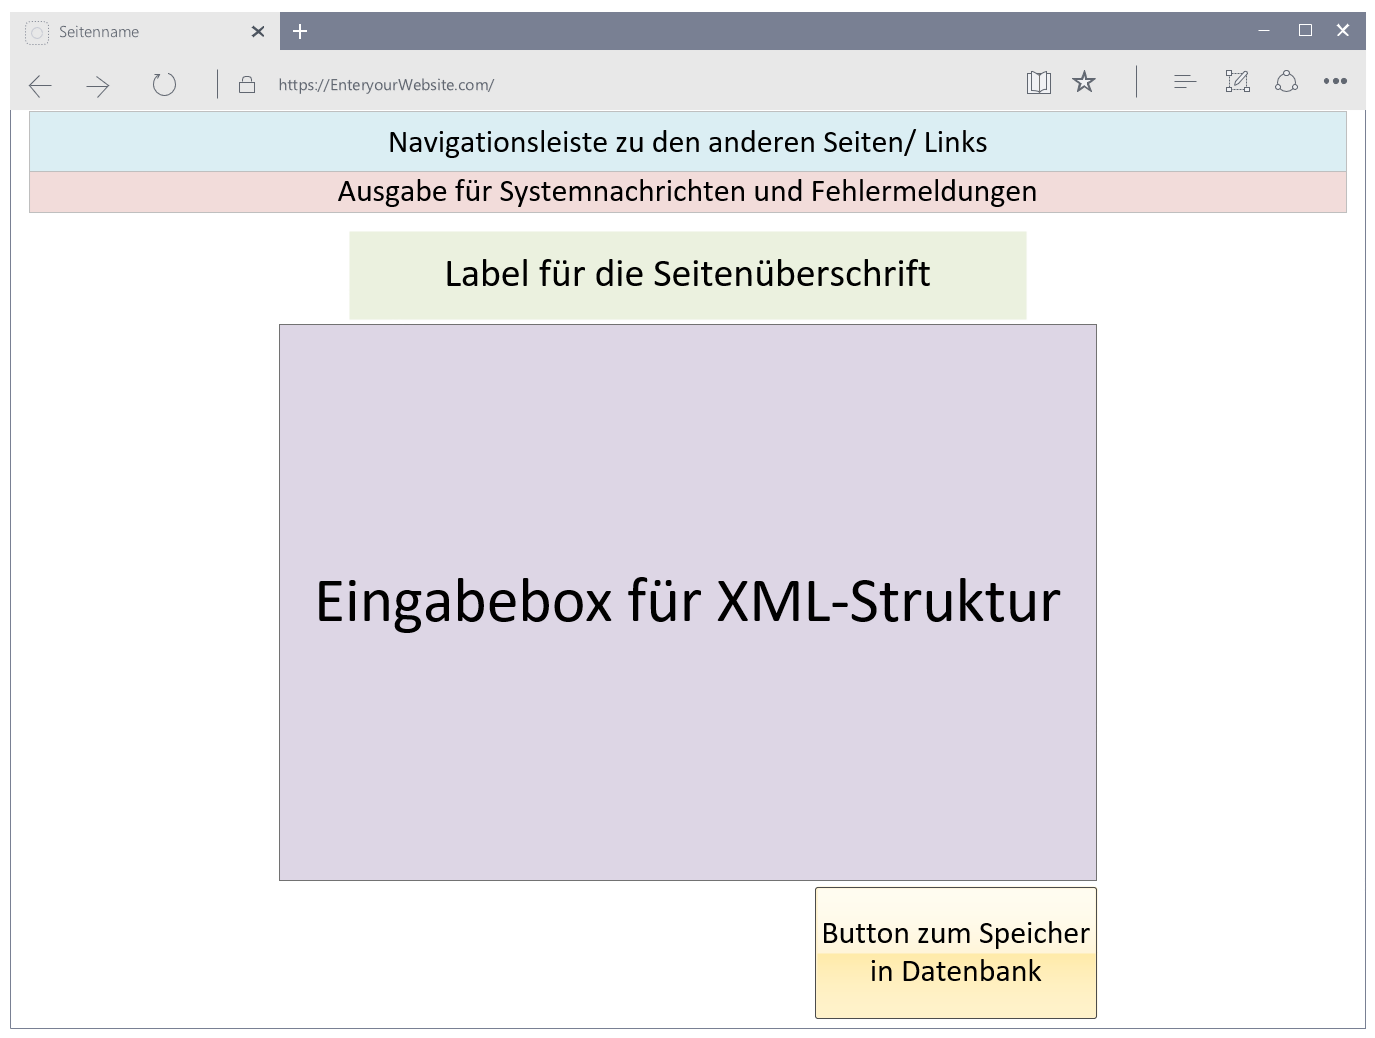
\includegraphics[width=0.95\textwidth]{Grafiken/Overlay_Einleseseite}
    \caption{Benutzeroberflächenentwurf der Seite zum einlesen der XML-Struktur}
    \label{fig: Benutzeroberflächenentwurf der Seite zum einlesen der XML-Struktur}
    {Quelle: Eigene Darstellung mit Microsoft Visio}
\end{figure}


\begin{figure}[H]
    \centering
    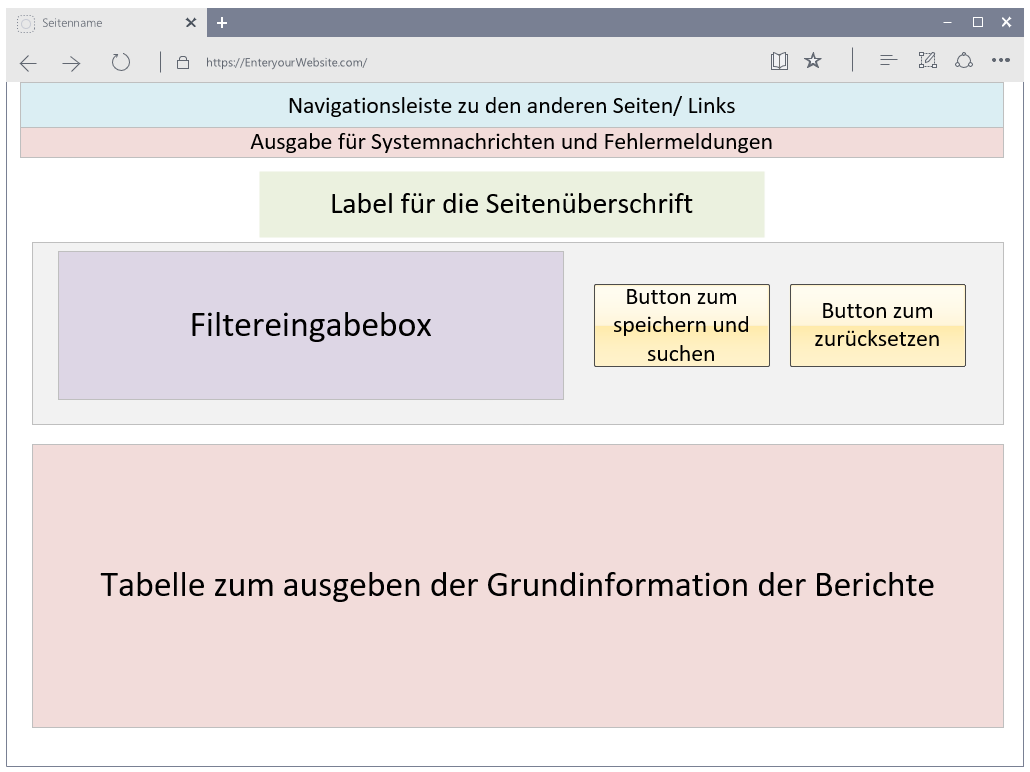
\includegraphics[width=0.95\textwidth]{Grafiken/Overlay_Tabellenseite}
    \caption{Benutzeroberflächenentwurf der Seite zum ausgeben der Berichtstabelle}
    \label{fig: Benutzeroberflächenentwurf der Seite zum ausgeben der Berichtstabelle}
    {Quelle: Eigene Darstellung mit Microsoft Visio}
\end{figure}


\begin{figure}[H]
    \centering
    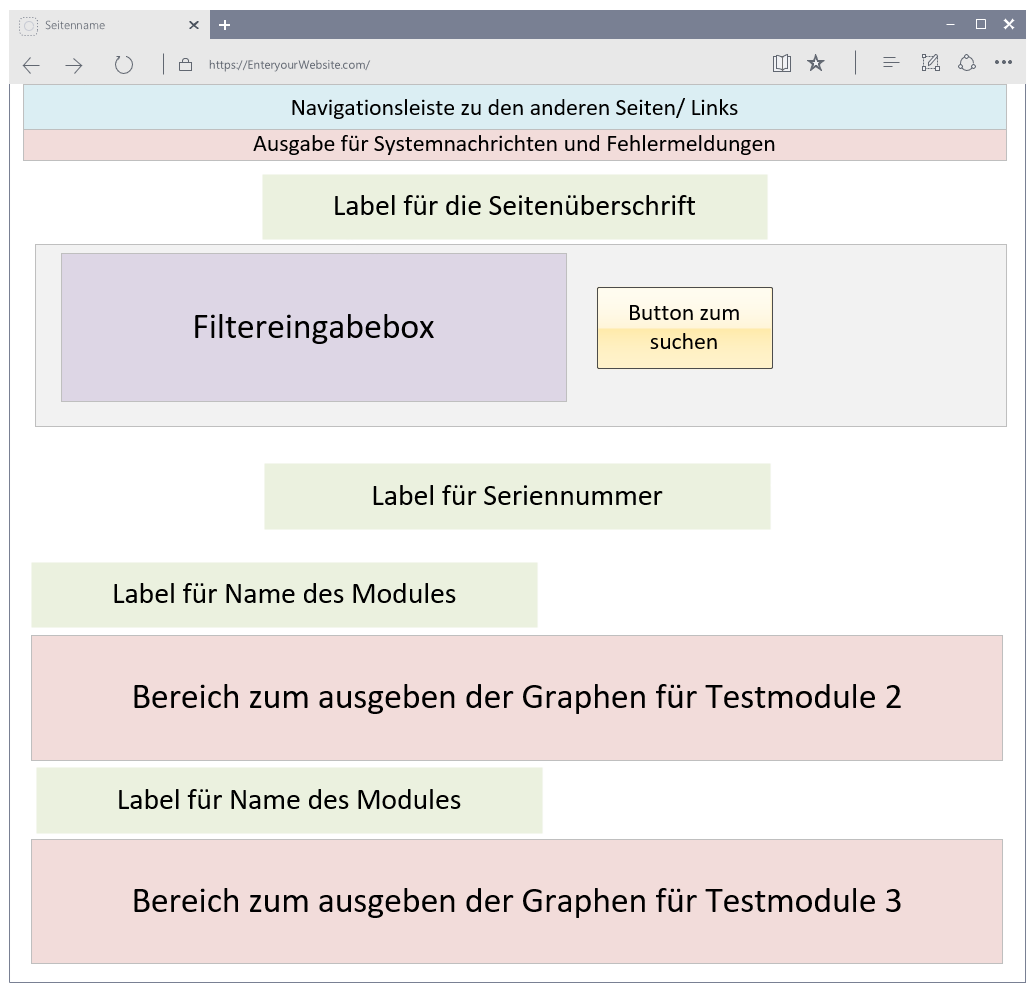
\includegraphics[width=0.95\textwidth]{Grafiken/Overlay_Ausgabeseite}
    \caption{Benutzeroberflächenentwurf der Seite zum ausgeben der Graphen}
    \label{fig: Benutzeroberflächenentwurf der Seite zum ausgeben der Graphen}
    {Quelle: Eigene Darstellung mit Microsoft Visio}
\end{figure}